%%%%%%%%%%%%%%%%%%%%%%%%
%% Sample use of the infthesis class to prepare a thesis. This can be used as 
%% a template to produce your own thesis.
%%
%% The title, abstract and so on are taken from Martin Reddy's csthesis class
%% documentation.
%%
%% MEF, October 2002
%%%%%%%%%%%%%%%%%%%%%%%%

%%%%
%% Load the class. Put any options that you want here (see the documentation
%% for the list of options). The following are samples for each type of
%% thesis:
%%
%% Note: you can also specify any of the following options:
%%  logo: put a University of Edinburgh logo onto the title page
%%  frontabs: put the abstract onto the title page
%%  deptreport: produce a title page that fits into a Computer Science
%%      departmental cover [not sure if this actually works]
%%  singlespacing, fullspacing, doublespacing: choose line spacing
%%  oneside, twoside: specify a one-sided or two-sided thesis
%%  10pt, 11pt, 12pt: choose a font size
%%  centrechapter, leftchapter, rightchapter: alignment of chapter headings
%%  sansheadings, normalheadings: headings and captions in sans-serif
%%      (default) or in the same font as the rest of the thesis
%%  [no]listsintoc: put list of figures/tables in table of contents (default:
%%      not)
%%  romanprepages, plainprepages: number the preliminary pages with Roman
%%      numerals (default) or consecutively with the rest of the thesis
%%  parskip: don't indent paragraphs, put a blank line between instead
%%  abbrevs: define a list of useful abbreviations (see documentation)
%%  draft: produce a single-spaced, double-sided thesis with narrow margins
%%
%% For a PhD thesis -- you must also specify a research institute:
\documentclass[phd,ilcc,twoside]{infthesis}

%% For an MPhil thesis -- also needs an institute
% \documentclass[mphil,ianc]{infthesis}

%% MSc by Research, which also needs an institute
% \documentclass[mscres,irr]{infthesis}

%% Taught MSc -- specify a particular degree instead. If none is specified,
%% "MSc in Informatics" is used.
% \documentclass[msc,cogsci]{infthesis}
% \documentclass[msc]{infthesis}  % for the MSc in Informatics

%% Master of Informatics (5 year degree)
% \documentclass[minf]{infthesis}

%% Undergraduate project -- specify the degree course and project type
%% separately
% \documentclass[bsc]{infthesis}
% \course{Artificial Intelligence and Psychology}
% \project{Fourth Year Project Report}

%% Put any \usepackage commands you want to use right here; the following is 
%% an example:
\usepackage{natbib}

%% Information about the title, etc.
\title{How I Did It}
\author{Victor von Frankenstein}

%% If the year of submission is not the current year, uncomment this line and 
%% specify it here:
% \submityear{1785}

%% Optionally, specify the graduation month and year:
% \graduationdate{February 1786}

%% Specify the abstract here.
\abstract{%
    This doctoral thesis will present the results of my work into the
    reanimation of lifeless human tissues.
}

%% Now we start with the actual document.
\begin{document}

%% First, the preliminary pages
\begin{preliminary}

%% This creates the title page
\maketitle

%% Acknowledgements
\begin{acknowledgements}
Many thanks to my mummy for the numerous packed lunches; and of course to
Igor, my faithful lab assistant.
\end{acknowledgements}

%% Next we need to have the declaration.
\standarddeclaration

%% Finally, a dedication (this is optional -- uncomment the following line if
%% you want one).
% \dedication{To my mummy.}

%% Create the table of contents
\tableofcontents

%% If you want a list of figures or tables, uncomment the appropriate line(s)
% \listoffigures
% \listoftables

\end{preliminary}

%%%%%%%%
%% Include your chapter files here. See the sample chapter file for the basic
%% format.

\chapter{Introduction}

In the psychometrics and educational literature different ideas for the evaluation of students have been developed. The variety of ideas is diverse, from models that accurately measure the student knowledge and proficiency in a topic to models that help in the quiz and item design. Although the ideas for these models typically arise from social sciences questions and assumptions, they are backed by statistical and mathematical tools that help to measure and interpret the results. This way, with the collaboration from both fields, a more detailed assessment and interpretation of the results can be provided for the students and instructors.


One idea for student assessment is through high-stake and low-stake tests. The basic idea is to apply one or more tests with different frequency level with the purpose to evaluate the knowledge and proficiency of the student for a topic or a set of topics. The frequency of the tests plays an important role in this text, in special the low-stake high-frequency quizzes. Frequent quizzes allow monitoring the student performance during the course, permitting the instructor to take actions based on the obtained information. On the other hand, in the high-stake quizzes, the instructor can only assess the knowledge of the students at the end of the course or when the high stake test is taken.

In this dissertation, some difficulties in the analysis of the low-stake high-frequency tests will be covered. Because the number of tests and the generated information increases, the time to evaluate each item and test difficulty is reduced, so a tool to quickly calculate them is required. Additionally, a tool to manage and constantly analyse the answers from the students is required, both to assess the required time for each quiz and to measure the performance of the group and particular students. All of these having as an objective that the instructor could quickly respond to the needs of the students in the group \cite{payne2009information} \cite{moodle}.

For the first point, the estimation of the item difficulty parameter, the use of the Item Response Theory will be proposed, in special of the Rasch models. These models allow to calculate a difficulty parameter for each item and also to provide the student's ability parameter. The most interesting part of this model is that it makes comparable both sets of parameters. This information can potentially benefit the class instructors because they will have a tool to prepare the tests difficult according to the student's abilities. Furthermore, the instructors can perform Just in Time Teaching and adapt their tests difficulties and necessities according to the specific group requirements. Currently, these models are implemented in R packages \footnote{For example in the eRm and the ltm packages.}.

For the second point, the management and constant analysis of student answers and test times, a new package is proposed. The main objective of this package is to ease the test analysis and make it feasible for instructors. This package is called \textit{lanalytics}, and its main objective is to administer and analyse quizzes in different grouping levels: per person, per quiz and per group. To include the idea of quizzes administration, the package can create a quiz object and a course object. Then the instructors can export all the data from the quizzes as an R data file or *.csv file. Then, if further analysis is required, they simply have to read the data files to visualise it and make an analysis. The package includes different visualisation tools that work with these quiz and course objects.

To join this two ideas, the management and analysis of the test's information and the estimation of the item difficulty and student abilities, a user interface is proposed. This interface is named \textit{The lanalytics dashboard} and is implemented in Shiny R, that is completely free and open source. As it can be hosted on a web page, it can allow that users that are not familiar with R can have access to the lanalytics package and some functions of the eRm package. As building a comprehensive software that makes analyses data from a wide spectrum of sources is a very long task, this will be just a prototype for further future developments.

In the second chapter of this dissertation, the background for Just in Time Teaching (JiTT) and Item Response Theory (IRT) will be given. In specific, the Rasch models and the plots that will be used in the dashboard will be covered. Later, in the third chapter, the lanalytics package will be introduced, and the motivation for each of the generated plots will be explained. In the fourth chapter, the Shiny interface prototype will be presented, and each component will be explained. In the fifth chapter, a user experience evaluation of the Shiny interface will be documented. Finally, the conclusions and future work will be provided in the sixth chapter.

All this project is stored in Github. The URL of both the package and the dashboard is: \url{https://github.com/savrgg/lanalytics}
% \chapter{Background}

The item design is a topic in the assessment process of tests and quizzes for educational courses. A division of these tests can be introduced according to the quiz weight in the final grade and on its periodicity. This way, the high-stake quizzes are tests with low periodicity and a huge reward or penalty for the persons that take it \cite{salvador}. On the other hand, a more frequent version of these tests are usually under a low-stake idea \footnote{between more quizzes are made, then these are ponderated less in the final grade}, and then it is allowed to constantly measure the current status and progress of the students. Moreover, through analysing these quizzes, the instructor can have the opportunity to improve the quality of the items and to early detect anomalies in the current group. By analysing the low-stake quizzes, the instructor can find useful information about the current group. For example, if the group misinterpret some core concept for the course, then the instructor can spend more time. Additionally, another factor that can be important is the questions formulations. If some anomaly is detected in the analysis of the answers and the answering time, then the instructor can review the issue in this item. All of these analyses are important because every course has a limited class time, so it is a good idea to spend it on topics or applications that have been problematic for the group. This idea of adapt the class with every quiz application is called Just In Time Teaching (JiTT) \cite{jitt} and will be explored later.

In the first section of this chapter a brief introduction of the Just in Time Teaching is presented, then a popular method to analyse item-based quizzes is discussed: the Rasch model. This is a model that helps the instructors to find a numerical representation of the difficulty of an item. Also, it finds a numerical representation of the individual ability of every student in the group \cite{bond2015applying}. The interesting point about this method is that it constructs an ability value per student that is comparable with the difficulty value of the item. This way the instructor can determine the level of the quiz not only based on the difficulty of the items, but also on the particular abilities of the current students. This model is explored in the second section of this chapter. 

\section{Just in Time Teaching}

When using low stake-frequent quizzes, the instructor can be aware of the current general performance of the group to make more emphasis in conflictive concepts and applications. Furthermore, the instructor can prepare the contents of the next class based on the extracted information from the analysis. For example, if the next class material requires the understanding of some core concepts, and the group is not experienced with them, then the professor can take some time to explain them. This class adaptation of the class according to the detected needings is called Just in Time Teaching \cite{jitt}.

\section{Item response theory (IRT)}

\subsection{Latent and observable variables}

The difference between an observable and a no observable variable relies on the capacity of being directly measured or recorded \cite{everett2013introduction}. The no observable variables are commonly called latent or hidden variables. In the models that have hidden parameters, the inference is not performed as usual, but it needs to be done through information from the observable variables. Examples of latent variables in social sciences are the public opinion, the social class, and the verbal ability \cite{everett2013introduction}. Neither of these variables is directly observed, but are inferred from others quantitative or qualitative variables. For example, the verbal ability can be inferred from tests that involve characteristics of what we think creates the verbal ability.

\subsection{Latent Variable Models}

In general, many statistical models use latent variables in its definitions, for example, the Gaussian mixture models \cite{bishop2006pattern} in which it is assumed that each observation corresponds to one class, but this class is unobserved (usually a subpopulation inside a population). Then the joint probability distribution of the observed variables and this unique hidden variable can be specified as \cite{bishop2006pattern}:

\begin{equation}
\label{eq:chap2_1}
p(x_{o}, x_{h}) = p(x_{o} | x_{h}) p(x_{h})
\end{equation}

With $x_{o}$ the set of observable variables and $x_{h}$ the set of hidden variables. In the above equation, the conditional probability given some specific class (hidden variable) $x_{h} = k$ is normally distributed. Then the model estimates the probability of belonging given some specific class $k$ as follows:

\begin{equation}
\label{eq:chap2_2}
p(x_{o} | x_{h} = k) = N(\mu_k, \sigma_k)
\end{equation}

Another popular class of methods is the Hidden Markov Models \cite{bishop2006pattern}, which are quite similar to the normal Markov Models, but the transition probability is now between the hidden variables instead of the visible ones. Then another probability to link the observable and hidden variables is defined and is known as the emission probability \footnote{In this example, there is one hidden variable per visible variable and are assumed to be discrete.}:

\begin{equation}
p(x_{o}, x_{h}) = p(x_{o_1} | x_{h_1}) p(x_{h_1}) \prod_{i =2}^n p(x_{o_i} | x_{h_i}) p(x_{h_i} | x_{h_{i-1}})
\end{equation}

Besides these models that are directly defined with latent variables, there are others that can be expressed with a latent variable structure, such as the commonly used Singular Value Decomposition \cite{friedman2009elements}. As can be observed, one common aspect of the latent variable models is that the joint probabilities can be represented in terms of a conditional distribution of the observed variables given the hidden variables. Then the observed variables are conditionally independent given the hidden variables \cite{everett2013introduction}:

\begin{equation}
p(x_{o} | x_{h}) = p(x_{o_1}| x_{h})*p(x_{o_2}| x_{h}) * ...*p(x_{o_n}| x_{h})
\end{equation}

Furthermore, these latent variable models can be classified according to the observable and latent variables (continuous or discrete). When the latent variable is considered a continuous variable, we can consider two well-known families of models \footnote{although there are more families of models, but these two are closely related to the topic} \cite{everett2013introduction}:

\begin{itemize}
\item{Factor analysis models (continuous observed variable)}
\item{Item response theory models (discrete observed variable)}
\end{itemize}

In the \textit{Factor Analysis Models} the observed variable is continuous. Then the latent variables are used to explain the variability of the observed variables. Commonly the number of latent variables is less than the number of observed variables. Formally, the factor analysis can be described as \cite{pmr}:

\begin{equation}
x_{o} = Ax_{h} + \mu + \epsilon
\end{equation}

where:

\begin{itemize}
\item{$x_{o} \in \mathbb{R}^{n}$ is the vector of observable variables}
\item{$x_{h} \in \mathbb{R}^{m}$ is the vector of hidden variables and is assumed to be normally distributed $x_{h} \sim N(0, I_m)$}
\item{$\mu \in \mathbb{R}^{n}$ is a constant vector that represents the mean of the data}
\item{$\epsilon \in \mathbb{R}^{n}$ is called the noise term. It is normally distributed $\epsilon \sim N(0, \Phi)$ with $\Phi$ diagonal}
\item{$A \in \mathbb{R}^{n \times m}$ is called the factor loading matrix.}
\end{itemize}

In this model is important to remark that the observed variables are conditionally independent given the hidden variables in $x_{h}$:

\begin{equation}
p(x_{o_1}, ... , x_{o_n}| x_{h}) = p(x_{o_1}| x_{h})*p(x_{o_2}| x_{h}) * ...*p(x_{o_n}| x_{h})
\end{equation}

In the \textit{Item Response Theory (IRT) models} the observed variables are discrete. This is useful because we can use it in models where the observed variables are inherently ordinal or categorical, for example in multiple choice questions with more than one correct answer (polytomous variables), or questions that can be scored as correct or incorrect (dichotomous or binary variables).

In the IRT models the hidden variable is continuous and is called a \textit{latent trait} and it usually represents the ability of the test takers. One of the most common models is the Rasch model that will be introduced in the next section.

\section{The Rasch model (RM)}

\subsection{The sigmoid function}

To explain the Rasch model, we are going to introduce the sigmoid function (which receive the name because of the \textit{S} shaped form). This function has the equation:

\begin{equation}\label{eq:rasch1}
 sigmoid(x) = \frac{1}{1+\exp(-x)}
\end{equation}
\vspace{2 mm}

The domain of this function is $(-\infty, \infty)$, and as can be shown, the limit to $-\infty$ is $0$ and the limit to $\infty$ is 1. In consequence, this expression is always bounded between (0,1), as showed in the \cref{img:sigmoid1}. This is very similar to the range of probability. \footnote{Except that the probability can take the values of 0 and 1}. Because of the last property, this curve is commonly used to model probabilities regarding some independent variable \textbf{x} \footnote{For now, let's assume that \textbf{x} is one dimensional}. For example, in the logistic regression, the curve is modelled in terms of $Z = B^T X$ where $B$ is a vector of parameters, and $X$ is the matrix that contains the regressors.

\begin{figure}[ht!]
  \centering
  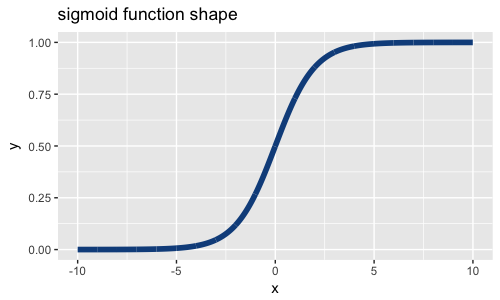
\includegraphics[width=.75\linewidth]{img/sigmoid.png}
  \caption{Sigmoid function. The domain of this function is $(-\infty, \infty)$ and the range $(0,1)$}
  \label{img:sigmoid1}
\end{figure}

Now, for the Rasch models, we need to analyse further the properties of the sigmoid function. If we subtract some positive scalar \textbf{a} to \textbf{x} in the equation \ref{eq:rasch1} then it result that the curve in \cref{img:sigmoid2} moves to the right, and the value of the sigmoid function decrease. Equivalently, if we add the same positive scalar \textbf{a}, then the curve moves to the left.

\begin{figure}[ht!]
  \centering
  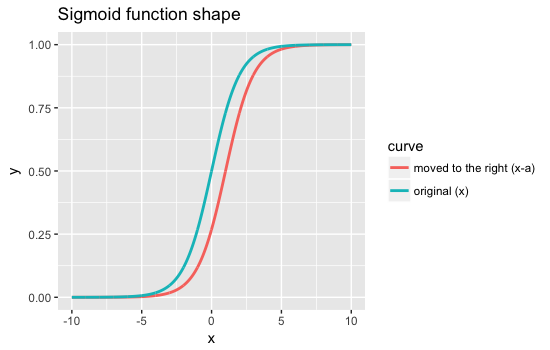
\includegraphics[width=.75\linewidth]{img/sigmoid_left.png}
  \caption{Effect of the variable \textbf{a} in the sigmoid function.}
  \label{img:sigmoid2}
\end{figure}


This idea is close to another formulation of the sigmoid function, which now can have two variables instead of one (\textbf{x,a}). With this modification, the domain and the range are the same. As mentioned before, the sigmoid function can be used to model a probability, that is, a continuous variable in the range [0,1], so then it is equivalent to a regression problem \footnote{More generally of a generalized linear model} \cite{friedman2009elements}. Now in terms of a classification problem (binary or dichotomous variable), this can be interpreted as the probability to belong to one of the two classes \footnote{Further generalizations for the polytomous case can be done.}. Then, the expression can be expressed as:

\begin{equation}
\begin{aligned}
\label{eq:rasch2}
 P(y = 1 | x,a) =& \frac{1}{1+\exp(-(x-a))} \\[2.5ex]
 =& \frac{\exp(x-a)}{1+\exp(x-a)}
\end{aligned}
\end{equation}

Where y is the binary variable. This basic idea is what support the basics of the Rasch model for dichotomous data.

\subsection{Rasch model}
Now, given this background, we can proceed with the definition of the Rasch model. From the last section, we can remember that the IRT models have a continuous latent variable (latent trait or ability) and an observable set of variables. In the next example, let's assume that this variable is binary and that the sigmoid function represents the probability of belonging to one of these classes.

\begin{equation}
  P(A_{rc} = 1 | \theta_r, \beta_c) = \frac{\exp(\theta_r - \beta_c)}{1+\exp(\theta_r - \beta_c)}
\end{equation}
Where:
\begin{itemize}
\item{$A$ is a matrix where the rows represent the persons and the columns the question of the quiz.}
\item{$A_{rc} \in \{0,1\}$ is the entry $(r,c)$ of the matrix $A$. This entry is a binary variable that represents the answer to the item $c$ of the person $r$. $0$ means that the person answers incorrectly and $1$ that answers correctly.}
\item{$\theta_r \in (-\infty, \infty)$ is the ability or trait of the person $r$.}
\item{$\beta_c \in [0, \infty)$ is the difficulty of the item $c$.}
\end{itemize}

Now, interpreting the result of the last subsection, if the parameter $\beta_c$ (difficulty) increases, then the sigmoid curve moves to the right leading to a decrease in the probability of getting correct the question. As in many statistical models, the problems rely on the parameter inference. For this reason, the author defines two auxiliary variables named \textit{Raw Scores}. Each of these scores is the marginalization of $A_{rc}$ with respect to the variables $r$ and $c$. Then each raw score depends only on one variable:

\begin{itemize}
\item{\textbf{Raw score per person:} $r_r = \sum_c A_{rc}$}
\item{\textbf{Raw score per item:} $s_c = \sum_r A_{rc}$}
\end{itemize}

The raw score per person is simply the sum of all the correct questions answered by each person; then it is a measure of the ability. On the other hand, the raw score per item is the sum of all persons that get correct that item, then it can be interpreted as the easiness of the item.

\subsection{The model assumptions}

According to \cite{demars2010item} \cite{mair2009extended} the Rasch model has the following assumptions:

\begin{itemize}
\item{ \textbf{1) Unidimensionality:}} The unidimensionality assumption is related to the dimensionality of the hidden parameters of the model. For the Rasch model, the ability parameter $\theta_{r}\in \mathbb{R}$ and the difficulty parameter $\beta_{c} \in \mathbb{R}$. Other models deal with multidimensional difficulty and ability parameters, but these will be not documented here.
\item{ \textbf{2) Conditional independence:}} The conditional independence is the same required for the latent variable models. This way, the observed item binary variables are independent among them given the parameters $\theta_{r}, \beta_c$
\item{ \textbf{3) Sufficiency of the raw score $r_r$:}} It is similar to the sufficiency in statistics. A statistics is sufficient if no other statistic provide some other information about the parameter with the sample.
\item{ \textbf{4) Monotonicity in the probability concerning the parameter $\theta_r$}}: That is, when having more ability, the probability of getting correct an item increase.

\end{itemize}

Due to the purpose of the text, the details about the tests for the assumptions will not be explained here. For more details about these tests, please consult \cite{demars2010item}.

\subsection{Item-parameter estimation}

In this section, a general review on the parameter estimation will be given. The basics of the item parameter estimation are based on the Maximum Likelihood Estimator, but according to \cite{mair2009extended} there are three ways to estimate the parameters:

\textbf{Joint Maximum likelihood Estimation (JML)}

The joint likehood formula of $\theta_r$ and $\beta_c$ is \cite{wright1969procedure} \cite{mair2009extended}:

\vspace{5 mm}

\begin{equation}
\begin{aligned}
L_{joint} =& \frac{\exp(\theta_r - \beta_c)^{\sum_c \sum_r a_{rc}}}{\prod_r \prod_i (1 + \exp(\theta_r - \beta_c))} \\[3.5ex]
    =& \frac{\exp(\sum_c \sum_r a_{rc} \theta_r) \exp(-\sum_c \sum_v a_{rc}\beta_c))}{\prod_r \prod_c (1 + \exp(\theta_r - \beta_c))} \\[3.5ex]
    =& \frac{\exp(\sum_r \theta_r r_r) \exp(-\sum_c \beta_c s_c)}{\prod_r \prod_c (1 + \exp(\theta_r - \beta_c))}
\end{aligned}
\end{equation}

\vspace{8 mm}

with $r_r = \sum_c A_{rc}$ and $s_c = \sum_r A_{rc}$. As reported in \cite{haberman1977maximum}, these estimation for the item parameters are not consistent when the number of the sample increases (there is one parameter per person, so it can increase too much).

\vspace{5 mm}

\textbf{Marginal Maximum likelihood Estimation (MML)}

If we integrate the person parameter, the joint distribution can be marginalised, and the parameters can be estimated via the Expected-Maximization algorithm \cite{bock1981marginal} \cite{mair2009extended}:

\vspace{5 mm}

\begin{equation}
L_{marg} = \prod_r \left[ \exp(-\sum_c \beta_c s_c) \int \frac{\exp(\theta_r)}{\prod_c^k (1 + exp(\theta-\beta_c)} dG(\theta)  \right]^{n_r}
\end{equation}

\vspace{5 mm}

Where it is assumed that the person parameter follows a predefined distribution. The expected maximisation algorithm is an algorithm that helps to maximise the likelihood of difficult problems. The idea is to include latent variables to make easier the maximisation process. For more information, this method is well documented in different texts \cite{friedman2009elements} \cite{bishop2006pattern}.

\vspace{5 mm}

\textbf{Conditional Maximum likelihood Estimation (CML)}

The third idea is to condition the joint likelihood on $r_r$ \cite{mair2009extended} (that is, conditioned on a sufficient statistic):

\vspace{5 mm}
\begin{equation}
L_{cond}= \frac{\exp(-\sum_r \beta_c s_c)}{\prod_r \sum_{x|r} ( -\exp(\sum_r x_r \beta_c)}
\end{equation}
\vspace{5 mm}

This way the parameters of the persons do not appear in the conditioning formula. 

\subsection{The Item Characteristic Curve (ICC)}

Now the question is how to plot the Rasch model. One way to do it is called the Item Characteristic Curve where we can display one item per curve. 

We already have the item and the person parameter, so we can calculate the probability of answering correctly one specific item for one specific person. If we make a plot where in the y-axis is the probability of getting correct this particular item and in the x-axis the person parameter and put one point per person. Then, the parameters of a sigmoid function are adjusted minimising the residuals between the individual points and this sigmoid function. This way we can have an Item Characteristic Curve as a representation of the model expectation \cite{demars2010item}:

\begin{figure}[ht!]
  \centering
  \includegraphics[width=.85\linewidth]{img/rasch_ICC.png}
  \caption{Item Characteristic Curve. Each curve represent one item.}
  \label{img:rasch_icc}
\end{figure}

The plot \cref{img:rasch_icc} plot is useful because we do not have to analyse all the abilities parameter of the persons, just one function that was fitted with all of these points. This way, we can easily identify which item was the most difficult. It is easy to identify that the leftmost curve is the easiest question and the rightmost curve the most difficult. 

\newpage

\subsection{The Person-Parameter plot (PPP)}
From the inference, we know the exact value of each person parameter, but now we have to answer how does this parameter be related to an observable variable. To answer this question, the Person-parameter plot maps the relation between the values of the ability parameter versus the number of correct answers of each person. This way we can have an idea of the relationship between the latent ability variable and the observable raw scores \cite{bond2015applying}:

\begin{figure}[ht!]
  \centering
  \includegraphics[width=.75\linewidth]{img/rasch_person.png}
  \caption{Rash model: person parameters. This plot shows the monotone relationship between the raw score per person and the value of the person parameter.}
  \label{img:rasch_person}
\end{figure}

\begin{table}[ht!]
\centering
\caption{Raw score per person and the person parameter.}
\label{tbl:person_pars}
\begin{tabular}{|l|l|l|}
\hline
\textbf{Person raw scores} & \textbf{\begin{tabular}[c]{@{}l@{}}Estimate person\\ parameter\end{tabular}} & \textbf{Std. Error} \\ \hline
5                         & -0.1963                                                                      & 0.6355              \\ \hline
6                          & 0.2050                                                                       & 0.6347              \\ \hline
7                          & 0.6182                                                                       & 0.6546              \\ \hline
8                          & 1.0750                                                                       & 0.7028              \\ \hline
9                          & 1.6339                                                                       & 0.8043              \\ \hline
10                          & 2.4685                                                                       & 1.0662              \\ \hline
\end{tabular}
\end{table}

In the \cref{img:rasch_person} we can see the raw scores and the person parameter from a synthetic dataset \footnote{the creation of this synthetic dataset are explained in chapter 4}. In this synthetic dataset, there were 11 questions, but the maximum raw score was 10. In the graph, we can observe that this relation is monotone. The idea is that between the number of correct answers increases, the student is more skilled.  \cite{bond2015applying}. 

\subsection{The Person-Item Map (PIM)}

Now, to show the relationship between the person parameters and the item parameters, the Person-Item map was created. In the uppermost part of this plot, it is shown the histogram of the person parameters regarding the latent dimension. We can see that the mode of this histogram was in the values $1.6339$ and $1.0750$ that correspond to eight and nine correct answers (see \cref{tbl:person_pars}). Also in the central part of the plot, we can observe the item parameters values (also regarding the same latent dimension).

This plot is interesting and useful because we can determine if the difficulty of the topics were lower for the ability of the students. In this synthetic example and the Person-Item map (\cref{img:rasch_personitem}), we can see that the difficulty of the topics are on the left side of the plot (most of them are below 0.6182 in the latent dimension), while the ability parameters of the students are in the right zone (most of them are above 0.6182 in the latent dimension). Then, in general terms in this example, the students were very skilled, and their ability was above the item difficulty. This is quite straightforward to deduce from the synthetic data set because to generate the answers, the probability to get right one question was at least 50\% for all items and students.

\begin{figure}[ht!]
  \centering
  \includegraphics[width=.75\linewidth]{img/rasch_personitem.png}
  \caption{Rasch model: Person-Item map}
  \label{img:rasch_personitem}
\end{figure}

%% ... etc ...

%%%%%%%%
%% Any appendices should go here. The appendix files should look just like the
%% chapter files.
\appendix
\include{appendix1}
%% ... etc...

%% Choose your favourite bibliography style here.
\bibliographystyle{apalike}

%% If you want the bibliography single-spaced (which is allowed), uncomment
%% the next line.
% \singlespace

%% Specify the bibliography file. Default is thesis.bib.
\bibliography{thesis}

%% ... that's all, folks!
\end{document}
